\chapter{Approach And Methods} % Chapter title

\label{chapter:approach_and_methods} % For referencing the chapter elsewhere, use \ref{chapter:computational_neuro} 

\def \blochwidth {0.3}
%\newcommand{\crzgate}{$\mathrm{CR_Z}$}
\newcommand{\plani}{$\mathcal{P}_i$}
\newcommand{\planj}{$\mathcal{P}_j$}
\newcommand{\querya}{$\mathcal{Q}_a$}
\newcommand{\queryb}{$\mathcal{Q}_b$}

% table cell head
\renewcommand{\cellalign}{lc}
\renewcommand{\theadalign}{cc}
\renewcommand\theadgape{\Gape[4pt]}
\renewcommand\theadfont{\normalsize}
\renewcommand\cellgape{\Gape[5pt]}
\renewcommand*{\arraystretch}{1.2}
%----------------------------------------------------------------------------------------
\section{Multiple Query Optimization}

\subsection{Data acquisition}
\label{chapter:mqp_data_acquisition}

The problem, as defined in chapter \ref{chapter:fundamental_multiple_query_optimization}, consists of a combination of costs $c$ per plan $\mathcal{P}_i$ and savings $s$ per combination $
\left(\mathcal{P}_i,\mathcal{P}_j\right)_{i \neq j}$. These values are basic integer numbers, which for any cost $c$ is in range [1,$x$] and for any saving $s$ in range [$y$,0]. As shown in chapter \ref{chapter:theoretical_fundamentals}, there can be $n$ queries at any given time, each of which has $n_i$ plans. These allow for multiple combinations, which by themselves define the problem space $\mathcal{D}$ to traverse. To begin with, the problem generator from Fankhauser et al.\cite{fankhauser_multiple_2021} is used to generate a basic problem space $\mathcal{D}_2\times2$ consisting of 2 queries, each with 2 plans, as seen in figure \ref{figure:2d_problem_data}.

\begin{figure}[!h]
    \centering
    \begin{minted}{python}
        (2,
          [23, 47, 25, 11],
          {(0, 2): -6,
           (0, 3): -4,
           (1, 2): -13,
           (1, 3): -6})
    \end{minted}
    \caption{This is an automatically generated problem space $\mathcal{D}_2\times2$. The first number tells us how many queries there are. In this example, all queries have two plans. The second array contains the cost of running each plan. The third segment is a dictionary where the key symbolizes which plans are combined, and the value of the savings that can be had.}
    \label{figure:2d_problem_data}
\end{figure}

To facilitate the visualization of the problem, the plans omit the $\mathcal{Q}_i$ prefix and are numbered from $\mathcal{P}_0$ up to $\mathcal{P}_n$. For example in \ref{figure:2d_problem_data}, this would mean that query $\mathcal{Q}_0$ has plans $\mathcal{P}_0$ and $\mathcal{P}_1$, and query $\mathcal{Q}_1$ plans $\mathcal{P}_2$ and $\mathcal{P}_3$, which is visualized in figure \ref{figure:4_query_plans}.

\begin{figure}[!h]
    \centering


\tikzset{every picture/.style={line width=0.75pt}} %set default line width to 0.75pt        

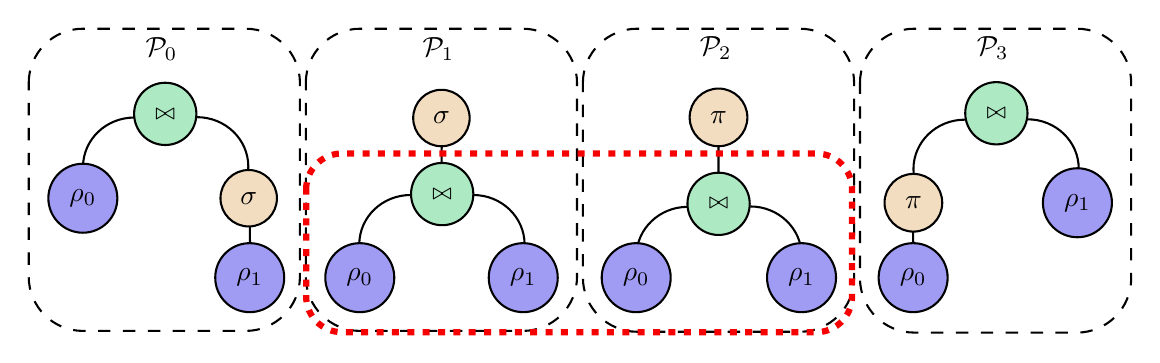
\begin{tikzpicture}[x=0.75pt,y=0.75pt,yscale=-1,xscale=1]
%uncomment if require: \path (0,517); %set diagram left start at 0, and has height of 517

%Rounded Rect [id:dp22693622189021267] 
\draw  [dash pattern={on 4.5pt off 4.5pt}] (105.33,90.93) .. controls (105.33,76.5) and (117.03,64.8) .. (131.47,64.8) -- (209.87,64.8) .. controls (224.3,64.8) and (236,76.5) .. (236,90.93) -- (236,184.27) .. controls (236,198.7) and (224.3,210.4) .. (209.87,210.4) -- (131.47,210.4) .. controls (117.03,210.4) and (105.33,198.7) .. (105.33,184.27) -- cycle ;
%Shape: Arc [id:dp9541025627566715] 
\draw  [draw opacity=0] (131.49,131.2) .. controls (131.6,118.14) and (142.63,107.59) .. (156.22,107.59) -- (156.22,131.41) -- cycle ; \draw   (131.49,131.2) .. controls (131.6,118.14) and (142.63,107.59) .. (156.22,107.59) ;  
%Shape: Arc [id:dp281513038224523] 
\draw  [draw opacity=0] (186.4,107.41) .. controls (200.06,107.41) and (211.13,118.07) .. (211.13,131.22) .. controls (211.13,132.92) and (210.94,134.58) .. (210.59,136.17) -- (186.4,131.22) -- cycle ; \draw   (186.4,107.41) .. controls (200.06,107.41) and (211.13,118.07) .. (211.13,131.22) .. controls (211.13,132.92) and (210.94,134.58) .. (210.59,136.17) ;  
%Straight Lines [id:da9126122398038725] 
\draw    (211.93,172.52) -- (211.92,159.12) ;
%Rounded Rect [id:dp19864875982463825] 
\draw  [dash pattern={on 4.5pt off 4.5pt}] (238.83,90.93) .. controls (238.83,76.5) and (250.53,64.8) .. (264.97,64.8) -- (343.37,64.8) .. controls (357.8,64.8) and (369.5,76.5) .. (369.5,90.93) -- (369.5,184.27) .. controls (369.5,198.7) and (357.8,210.4) .. (343.37,210.4) -- (264.97,210.4) .. controls (250.53,210.4) and (238.83,198.7) .. (238.83,184.27) -- cycle ;
%Shape: Arc [id:dp623273643179123] 
\draw  [draw opacity=0] (264.59,168.54) .. controls (264.7,155.48) and (275.73,144.92) .. (289.32,144.92) -- (289.32,168.74) -- cycle ; \draw   (264.59,168.54) .. controls (264.7,155.48) and (275.73,144.92) .. (289.32,144.92) ;  
%Shape: Arc [id:dp7769680524712608] 
\draw  [draw opacity=0] (319.5,144.92) .. controls (333.16,144.92) and (344.23,155.58) .. (344.23,168.74) -- (319.5,168.74) -- cycle ; \draw   (319.5,144.92) .. controls (333.16,144.92) and (344.23,155.58) .. (344.23,168.74) ;  
%Straight Lines [id:da8996795114234546] 
\draw    (304.18,135.28) -- (304.33,120.33) ;
%Rounded Rect [id:dp7958670756995907] 
\draw  [dash pattern={on 4.5pt off 4.5pt}] (372.33,90.93) .. controls (372.33,76.5) and (384.03,64.8) .. (398.47,64.8) -- (476.87,64.8) .. controls (491.3,64.8) and (503,76.5) .. (503,90.93) -- (503,184.67) .. controls (503,199.1) and (491.3,210.8) .. (476.87,210.8) -- (398.47,210.8) .. controls (384.03,210.8) and (372.33,199.1) .. (372.33,184.67) -- cycle ;
%Shape: Arc [id:dp2653269087913137] 
\draw  [draw opacity=0] (398.09,174.24) .. controls (398.2,161.18) and (409.23,150.62) .. (422.82,150.62) -- (422.82,174.44) -- cycle ; \draw   (398.09,174.24) .. controls (398.2,161.18) and (409.23,150.62) .. (422.82,150.62) ;  
%Shape: Arc [id:dp4205447304867884] 
\draw  [draw opacity=0] (453,150.44) .. controls (453,150.44) and (453,150.44) .. (453,150.44) .. controls (466.66,150.44) and (477.73,161.1) .. (477.73,174.26) -- (453,174.26) -- cycle ; \draw   (453,150.44) .. controls (453,150.44) and (453,150.44) .. (453,150.44) .. controls (466.66,150.44) and (477.73,161.1) .. (477.73,174.26) ;  
%Straight Lines [id:da9337925646863472] 
\draw    (437.68,134.98) -- (437.67,121.58) ;
%Rounded Rect [id:dp8024574861780045] 
\draw  [dash pattern={on 4.5pt off 4.5pt}] (505.83,90.93) .. controls (505.83,76.5) and (517.53,64.8) .. (531.97,64.8) -- (610.37,64.8) .. controls (624.8,64.8) and (636.5,76.5) .. (636.5,90.93) -- (636.5,185.07) .. controls (636.5,199.5) and (624.8,211.2) .. (610.37,211.2) -- (531.97,211.2) .. controls (517.53,211.2) and (505.83,199.5) .. (505.83,185.07) -- cycle ;
%Shape: Arc [id:dp2988707343502508] 
\draw  [draw opacity=0] (532.25,137.94) .. controls (531.82,136.18) and (531.59,134.33) .. (531.59,132.44) .. controls (531.59,119.28) and (542.66,108.62) .. (556.32,108.62) -- (556.32,132.44) -- cycle ; \draw   (532.25,137.94) .. controls (531.82,136.18) and (531.59,134.33) .. (531.59,132.44) .. controls (531.59,119.28) and (542.66,108.62) .. (556.32,108.62) ;  
%Shape: Arc [id:dp10478086547979326] 
\draw  [draw opacity=0] (586.5,108.44) .. controls (586.5,108.44) and (586.5,108.44) .. (586.5,108.44) .. controls (600.16,108.44) and (611.23,119.1) .. (611.23,132.26) .. controls (611.23,132.73) and (611.21,133.2) .. (611.19,133.66) -- (586.5,132.26) -- cycle ; \draw   (586.5,108.44) .. controls (586.5,108.44) and (586.5,108.44) .. (586.5,108.44) .. controls (600.16,108.44) and (611.23,119.1) .. (611.23,132.26) .. controls (611.23,132.73) and (611.21,133.2) .. (611.19,133.66) ;  
%Straight Lines [id:da5382439939318251] 
\draw    (531.48,173.38) -- (531.47,159.98) ;

%Rounded Rect [id:dp22736885699089981] 
\draw  [color={rgb, 255:red, 246; green, 1; blue, 1 }  ,draw opacity=1 ][dash pattern={on 2.53pt off 3.02pt}][line width=2.25]  (239,142.14) .. controls (239,132.63) and (246.71,124.92) .. (256.22,124.92) -- (484.78,124.92) .. controls (494.29,124.92) and (502,132.63) .. (502,142.14) -- (502,193.78) .. controls (502,203.29) and (494.29,211) .. (484.78,211) -- (256.22,211) .. controls (246.71,211) and (239,203.29) .. (239,193.78) -- cycle ;

% Text Node
\draw (427.17,67.23) node [anchor=north west][inner sep=0.75pt]    {$\mathcal{P}_{2}$};
% Text Node
\draw  [fill={rgb, 255:red, 242; green, 221; blue, 192 }  ,fill opacity=1 ]  (437.67, 107.53) circle [x radius= 13.9, y radius= 13.9]   ;
\draw (437.67,107.53) node    {$\pi $};
% Text Node
\draw (560.67,67.23) node [anchor=north west][inner sep=0.75pt]    {$\mathcal{P}_{3}$};
% Text Node
\draw  [fill={rgb, 255:red, 242; green, 221; blue, 192 }  ,fill opacity=1 ]  (531.57, 148.65) circle [x radius= 13.9, y radius= 13.9]   ;
\draw (531.57,148.65) node    {$\pi $};
% Text Node
\draw  [fill={rgb, 255:red, 173; green, 234; blue, 195 }  ,fill opacity=1 ]  (437.71, 149.17) circle [x radius= 15, y radius= 15]   ;
\draw (437.71,149.17) node  [font=\footnotesize]  {$\bowtie $};
% Text Node
\draw  [fill={rgb, 255:red, 173; green, 234; blue, 195 }  ,fill opacity=1 ]  (571.54, 105.53) circle [x radius= 15, y radius= 15]   ;
\draw (571.54,105.53) node  [font=\footnotesize]  {$\bowtie $};
% Text Node
\draw  [fill={rgb, 255:red, 160; green, 156; blue, 243 }  ,fill opacity=1 ]  (398.01, 184.74) circle [x radius= 16.62, y radius= 16.62]   ;
\draw (398.01,184.74) node   [align=left] {$\displaystyle \rho _{0}$};
% Text Node
\draw  [fill={rgb, 255:red, 160; green, 156; blue, 243 }  ,fill opacity=1 ]  (477.67, 184.74) circle [x radius= 16.62, y radius= 16.62]   ;
\draw (477.67,184.74) node   [align=left] {$\displaystyle \rho _{1}$};
% Text Node
\draw  [fill={rgb, 255:red, 160; green, 156; blue, 243 }  ,fill opacity=1 ]  (531.44, 184.74) circle [x radius= 16.62, y radius= 16.62]   ;
\draw (531.44,184.74) node   [align=left] {$\displaystyle \rho _{0}$};
% Text Node
\draw  [fill={rgb, 255:red, 160; green, 156; blue, 243 }  ,fill opacity=1 ]  (610.59, 148.65) circle [x radius= 16.62, y radius= 16.62]   ;
\draw (610.59,148.65) node   [align=left] {$\displaystyle \rho _{1}$};
% Text Node
\draw (160.17,67.53) node [anchor=north west][inner sep=0.75pt]    {$\mathcal{P}_{0}$};
% Text Node
\draw (293.67,67.53) node [anchor=north west][inner sep=0.75pt]    {$\mathcal{P}_{1}$};
% Text Node
\draw  [fill={rgb, 255:red, 242; green, 221; blue, 192 }  ,fill opacity=1 ]  (304.17, 107.83) circle [x radius= 13.6, y radius= 13.6]   ;
\draw (304.17,107.83) node    {$\sigma $};
% Text Node
\draw  [fill={rgb, 255:red, 173; green, 234; blue, 195 }  ,fill opacity=1 ]  (304.54, 144.47) circle [x radius= 15, y radius= 15]   ;
\draw (304.54,144.47) node  [font=\footnotesize]  {$\bowtie $};
% Text Node
\draw  [fill={rgb, 255:red, 160; green, 156; blue, 243 }  ,fill opacity=1 ]  (264.84, 184.74) circle [x radius= 16.62, y radius= 16.62]   ;
\draw (264.84,184.74) node   [align=left] {$\displaystyle \rho _{0}$};
% Text Node
\draw  [fill={rgb, 255:red, 160; green, 156; blue, 243 }  ,fill opacity=1 ]  (343.59, 184.74) circle [x radius= 16.62, y radius= 16.62]   ;
\draw (343.59,184.74) node   [align=left] {$\displaystyle \rho _{1}$};
% Text Node
\draw  [fill={rgb, 255:red, 173; green, 234; blue, 195 }  ,fill opacity=1 ]  (171.11, 105.83) circle [x radius= 15, y radius= 15]   ;
\draw (171.11,105.83) node  [font=\footnotesize]  {$\bowtie $};
% Text Node
\draw  [fill={rgb, 255:red, 160; green, 156; blue, 243 }  ,fill opacity=1 ]  (131.41, 146.47) circle [x radius= 16.62, y radius= 16.62]   ;
\draw (131.41,146.47) node   [align=left] {$\displaystyle \rho _{0}$};
% Text Node
\draw  [fill={rgb, 255:red, 160; green, 156; blue, 243 }  ,fill opacity=1 ]  (211.81, 184.74) circle [x radius= 16.62, y radius= 16.62]   ;
\draw (211.81,184.74) node   [align=left] {$\displaystyle \rho _{1}$};
% Text Node
\draw  [fill={rgb, 255:red, 242; green, 221; blue, 192 }  ,fill opacity=1 ]  (211.32, 146.47) circle [x radius= 13.6, y radius= 13.6]   ;
\draw (211.32,146.47) node    {$\sigma $};


\end{tikzpicture}


    \caption{4 different query plans $\mathcal{P}_0$, $\mathcal{P}_1$ for query $\mathcal{Q}_0$ and $\mathcal{P}_2$, $\mathcal{P}_3$ for query $\mathcal{Q}_1$. The plans have different ordered instructions, which can save time during single execution or allow for more parallel savings.}
    \label{figure:4_query_plans}
\end{figure}

The plans from figure \ref{figure:4_query_plans} are built to best resemble the costs and savings defined in the data from figure \ref{figure:2d_problem_data}. It defines that the combination of $\mathcal{P}_1$ and $\mathcal{P}_2$ offers the greatest savings. In this case, the step that would warrant such savings would be $\rho_0\bowtie\rho_1$, that is present in both plans, and surrounded with a red rectangle. In every other case, there are preliminary operations that change the result so that it is not shareable by the plans. Nevertheless, one could still share the single steps $\rho_0$ and $\rho_1$, which in this case symbolize the loading of tables into memory. 

\newpage

The problem space from figure \ref{figure:2d_problem_data} is used for direct comparison between our solution and the solution of Fankhauer et al.\cite{fankhauser_multiple_2021}. As one cannot assume that real life problems will always be limited to 2 queries with 2 problems each, the problem generator is enhanced to allow for any number of queries, each of which with their own number of plans, as shown in figure \ref{figure:nd_problem_data}.

\begin{figure}[!h]
    \centering
    \begin{minted}{python}
        ([2, 3, 2],
          [21,  1, 36, 16, 33, 42,  7],
          {(0, 2): -7,
           (0, 3): -13,
           (0, 4): -14,
           (0, 5): -6,
           (0, 6): 0,
           (1, 2): -18,
           (1, 3): -12,
           (1, 4): -17,
           (1, 5): -14,
           (1, 6): -4,
           (2, 5): -5,
           (2, 6): -6,
           (3, 5): -20,
           (3, 6): -12,
           (4, 5): -10,
           (4, 6): 0})
    \end{minted}
    \caption{This is an automatically generated, $n$-dimensional problem space $\mathcal{D}$. The first array tells us how many plans each query has. This problem has 3 queries, two of which have 2 plans and one with 3 plans. Just like the problem from figure \ref{figure:2d_problem_data}, the second element is an array that contains the cost of each plan, and the third element, which is a dictionary, contains the combinations keys and their respective savings.}
    \label{figure:nd_problem_data}
\end{figure}

\newpage

\subsection{Circuit Design}

The design of the circuit is carefully modelled as to allow easier understanding of its behaviour. Initially, for any $n$ plans, the probabilities of each being the cheapest is unknown, which directly means they are all \emph{equally probable}. To create equal probabilities for all plans, an initial layer consisting of one \hgate\ per qubit is constructed, as illustrated in figure \ref{figure:4_qubit_circuit_with_h_gates}.

\begin{figure}[!h]
    \centering
    \scalebox{1.0}{
    \Qcircuit @C=1.0em @R=0.2em @!R { \\
	 	\nghost{{\mathcal{P}}_{0} :  } & \lstick{{\mathcal{P}}_{0} :  } \barrier[0em]{3} & \qw & \gate{\mathrm{H}} \barrier[0em]{3} & \qw & \qw & \qw\\
	 	\nghost{{\mathcal{P}}_{1} :  } & \lstick{{\mathcal{P}}_{1} :  } & \qw & \gate{\mathrm{H}} & \qw & \qw & \qw\\
	 	\nghost{{\mathcal{P}}_{2} :  } & \lstick{{\mathcal{P}}_{2} :  } & \qw & \gate{\mathrm{H}} & \qw & \qw & \qw\\
	 	\nghost{{\mathcal{P}}_{3} :  } & \lstick{{\mathcal{P}}_{3} :  } & \qw & \gate{\mathrm{H}} & \qw & \qw & \qw\\
	 	\nghost{} & \lstick{} & \ket{\psi_0} &  & \ket{\psi_1}\\
\\ }}
    \caption{A 4 qubit circuit (here the qubits are not denoted with $q_i$ but $\mathcal{P}_i$, which represent for each plan in the problem) for the problem defined in figure \ref{figure:2d_problem_data} consisting of only \hgate s to create an equal superposition across all plans}
    \label{figure:4_qubit_circuit_with_h_gates}
\end{figure}

\begin{equation}
    \centering
    \begin{split}
        \mathcal{P}_i =\ \ket{0} &=\ \ket{\psi_0} =\ \begin{pmatrix}1 \\ 0\end{pmatrix}\\
        \mathrm{H}\mathcal{P}_i =\ \mathrm{H}\ket{0} &=\ \frac{1}{\sqrt{2}}\ket{0} + \frac{1}{\sqrt{2}}\ket{1} =\ \begin{pmatrix}\frac{1}{\sqrt{2}} \\ \frac{1}{\sqrt{2}}\end{pmatrix} =\ \ket{\psi_1}\\
        |\bra{1}\ket{\psi_1}_{\mathrm{P}_0}|^2 &=\ \left|\frac{1}{\sqrt{2}}\right|^2 =\ 0.5\\
        |\bra{0}\ket{\psi_1}_{\mathrm{P}_0}|^2 &=\ \left|\frac{1}{\sqrt{2}}\right|^2 =\ 0.5\\
    \end{split}
    \label{equation:2d_problem_state_0_1}
\end{equation}

Whereas at position $\ket{\psi_0}$ all qubits have the state $\ket{0}$, after applying the \hgate s, all the qubits have the state $\frac{1}{\sqrt{2}}\ket{0} + \frac{1}{\sqrt{2}}\ket{1}$ at position $\ket{\psi_1}$. To assess that the circuit behaves correctly, measurement calculations for $\ket{0}$ and $\ket{1}$ are shown in equation \ref{equation:2d_problem_state_0_1}. 
\subsection{Cost Embedding}

The idea behind the design of the cost embedding onto the quantum circuit is relatively simple. The more expensive a single plan $\mathcal{P}_i$ is, the less its probability to be $1$ should be. To do this, a \rygate\ gate is used per qubit, which can change the probabilities towards $\ket{0}$ or $\ket{1}$. In the end, the probability for $\ket{1}$ should \emph{decrease} with a high cost in the problem space, and \emph{increase} with a low cost.

\newpage

\begin{figure}[!h]
    \centering
    \scalebox{1.0}{
    \Qcircuit @C=1.0em @R=0.2em @!R { \\
	 	\nghost{{q}_{0} :  } & \lstick{{\mathcal{P}}_{0} :  } & \gate{\mathrm{H}} & \gate{\mathrm{R_Y}\,(\mathrm{c_0})} \barrier[0em]{3} & \qw & \qw & \qw\\
	 	\nghost{{q}_{1} :  } & \lstick{{\mathcal{P}}_{1} :  } & \gate{\mathrm{H}} & \gate{\mathrm{R_Y}\,(\mathrm{c_1})} & \qw & \qw & \qw\\
	 	\nghost{{q}_{2} :  } & \lstick{{\mathcal{P}}_{2} :  } & \gate{\mathrm{H}} & \gate{\mathrm{R_Y}\,(\mathrm{c_2})} & \qw & \qw & \qw\\
	 	\nghost{{q}_{3} :  } & \lstick{{\mathcal{P}}_{3} :  } & \gate{\mathrm{H}} & \gate{\mathrm{R_Y}\,(\mathrm{c_3})} & \qw & \qw & \qw\\
	 	\nghost{} : & \lstick{{} } & & & \ket{\psi_2}& \\
    \\ }}
    \caption{The 4 qubit circuit from figure \ref{figure:4_qubit_circuit_with_h_gates} for the problem defined in figure \ref{figure:2d_problem_data} improved with cost encoding \rygate.}
    \label{figure:4_qubit_circuit_with_h_ry_gates}
\end{figure}

\begin{equation}
    \centering
    \begin{split}
        \mathrm{RY}(c_i)\mathrm{H}\mathcal{P}_i &=\ \begin{pmatrix} \cos{\frac{c_i}{2}} & -\sin{\frac{c_i}{2}} \\ \sin{\frac{c_i}{2}} & \cos{\frac{c_i}{2}} \end{pmatrix}\begin{pmatrix}\frac{1}{\sqrt{2}} \\ \frac{1}{\sqrt{2}}\end{pmatrix}\\
        \mathrm{RY}(c_i)\mathrm{H}\mathcal{P}_i &=\ \frac{1}{\sqrt{2}}\begin{pmatrix}\cos(\frac{c_i}{2}) - \sin(\frac{c_i}{2}) \\ \sin(\frac{c_i}{2}) + \cos(\frac{c_i}{2})\end{pmatrix} =\ \ket{\psi_2}\\
    \end{split}
    \label{equation:2d_problem_state_0_1}
\end{equation}

\begin{equation}
    \centering
    \begin{split}
        c_0 &=\ 0.5\\
        c_1 &=\ -0.5\\
        |\bra{0}\ket{\psi_2}_{\mathrm{P_0}}|^2 &=\ 0.2603 \\
        |\bra{1}\ket{\psi_2}_{\mathrm{P_0}}|^2 &=\ 0.7397 \\
        |\bra{0}\ket{\psi_2}_{\mathrm{P_1}}|^2 &=\ 0.7397 \\
        |\bra{1}\ket{\psi_2}_{\mathrm{P_1}}|^2 &=\ 0.2603 \\
    \end{split}
    \label{equation:2d_problem_state_measurements}
\end{equation}

As equation \ref{equation:2d_problem_state_measurements} shows, the opposite happens. This can be easily corrected by multiplying the cost with a factor of $-1$, with the corrected circuit shown in figure \ref{figure:4_qubit_circuit_with_h_neg_ry_gates}. Before the cost is applied, any qubit in the given circuit from figure \ref{figure:4_qubit_circuit_with_h_ry_gates} has the state shown in figure \ref{figure:q_sphere_no_cost}. Applying the cost factors, a high-cost \emph{increases} the chances of measuring $0$, as shown in figure \ref{figure:q_sphere_bad_cost} whereas a low-cost increases the chances of measuring a $1$, as demonstrate in figure \ref{figure:q_sphere_good_cost}. 


\begin{figure}[!h]
    \centering
    \scalebox{1.0}{
    \Qcircuit @C=1.0em @R=0.2em @!R { \\
	 	\nghost{{q}_{0} :  } & \lstick{{\mathcal{P}}_{0} :  } & \gate{\mathrm{H}} & \gate{\mathrm{R_Y}\,(-\mathrm{c_0})} \barrier[0em]{3} & \qw & \qw & \qw\\
	 	\nghost{{q}_{1} :  } & \lstick{{\mathcal{P}}_{1} :  } & \gate{\mathrm{H}} & \gate{\mathrm{R_Y}\,(-\mathrm{c_1})} & \qw & \qw & \qw\\
	 	\nghost{{q}_{2} :  } & \lstick{{\mathcal{P}}_{2} :  } & \gate{\mathrm{H}} & \gate{\mathrm{R_Y}\,(-\mathrm{c_2})} & \qw & \qw & \qw\\
	 	\nghost{{q}_{3} :  } & \lstick{{\mathcal{P}}_{3} :  } & \gate{\mathrm{H}} & \gate{\mathrm{R_Y}\,(-\mathrm{c_3})} & \qw & \qw & \qw\\
	 	\nghost{} : & \lstick{{} } & & & \ket{\psi_2}& \\
    \\ }}
    \caption{The 4 qubit circuit from figure \ref{figure:4_qubit_circuit_with_h_ry_gates} with negated parameter $c_i$, so that the probabilities move correctly according to the cost of each plan $\mathrm{P}_i$.}
    \label{figure:4_qubit_circuit_with_h_neg_ry_gates}
\end{figure}


\begin{figure}[!h]
    \centering
    \scalebox{\histogramwidth}{
        \includesvg{thesis/Appendices/Q_Sphere_State_h.svg}
    }
    \caption{A Q-Sphere showing the state of a single qubit (representing a plan $\mathcal{P}_i$), where the probabilities of $\ket{0}$ and $\ket{1}$ are equal.}
    \label{figure:q_sphere_no_cost}
\end{figure}

\begin{figure}[!h]
    \centering
    \scalebox{\histogramwidth}{
        \includesvg{thesis/Appendices/Bloch_Sphere_bad_cost.svg}
    }
    \caption{A Q-Sphere that shows the state of a single qubit (representing a plan $\mathcal{P}_i$), where the cost $0.5$ was embedded onto state \ref{figure:q_sphere_no_cost} and therefore the probability of a $\ket{0}$ increased.}
    \label{figure:bloch_sphere_bad_cost}
\end{figure}

\begin{figure}[!h]
    \centering
    \scalebox{\histogramwidth}{
        \includesvg{thesis/Appendices/Bloch_Sphere_good_cost.svg}
    }
    \caption{A Q-Sphere that shows the state of a single qubit (representing a plan $\mathcal{P}_i$), where the cost $-0.5$ was embedded onto state \ref{figure:q_sphere_no_cost} and therefore the probability of a $\ket{1}$ increased.}
    \label{figure:bloch_sphere_good_cost}
\end{figure}

\newpage

\subsection{Savings Embedding}

The savings follow roughly the same idea. Instead of a \rygate, the entanglement \crzgate\ is used to embed the savings each combination of plans has. For two plans \plani\ and \planj\ to be entangled, the rule \ref{equation:entanglement_rule} has to be true.

\begin{equation}
\centering
    \begin{split}
        \forall\  \mathcal{P}_i,\ \mathcal{P}_j,\ \mathcal{Q}_a,\ \mathcal{Q}_b &\in\ \mathcal{D}\ \\ 
        i \neq j \wedge\ a \neq b \wedge\ \left(\mathcal{P}_i\ \in\ \mathcal{Q}_a\ \wedge \mathcal{P}_j\ \notin\ \mathcal{Q}_a\right) &\wedge\ \left(\mathcal{P}_j\ \in\ \mathcal{Q}_b\ \wedge \mathcal{P}_i\ \notin\ \mathcal{Q}_b\right)\\
    \end{split}
    \label{equation:entanglement_rule}
\end{equation}


As defined for a problem space $\mathcal{D}$ in figure \ref{figure:2d_problem_data}, the savings themselves are negative. A circuit with all data embeddings is visualized in figure \ref{figure:4_qubit_circuit_with_h_ry_crz_gates}.

\begin{figure}[!h]
    \centering
    \scalebox{1.0}{
\Qcircuit @C=1.0em @R=0.2em @!R { \\
	 	\nghost{{q}_{0} :  } & \lstick{{\mathcal{P}}_{0}  :  } & \gate{\mathrm{H}} & \gate{\mathrm{R_Y}\,(\mathrm{-c_0})} & \ctrl{2} & \ctrl{3} & \qw & \qw \barrier[0em]{3} & \qw & \qw & \qw\\
	 	\nghost{{q}_{1} :  } & \lstick{{\mathcal{P}}_{1}  :  } & \gate{\mathrm{H}} & \gate{\mathrm{R_Y}\,(\mathrm{-c_1})} & \qw & \qw & \ctrl{1} & \ctrl{2} & \qw & \qw & \qw\\
	 	\nghost{{q}_{2} :  } & \lstick{{\mathcal{P}}_{2}  :  } & \gate{\mathrm{H}} & \gate{\mathrm{R_Y}\,(\mathrm{-c_2})} & \gate{\mathrm{R_Z}\,(\mathrm{s_{02}})} & \qw & \gate{\mathrm{R_Z}\,(\mathrm{s_{12}})} & \qw & \qw & \qw & \qw\\
	 	\nghost{{q}_{3} :  } & \lstick{{\mathcal{P}}_{3}  :  } & \gate{\mathrm{H}} & \gate{\mathrm{R_Y}\,(\mathrm{-c_3})} & \qw & \gate{\mathrm{R_Z}\,(\mathrm{s_{03}})} & \qw & \gate{\mathrm{R_Z}\,(\mathrm{s_{13}})} & \qw & \qw & \qw\\
	 	\nghost{ } & \lstick{ } & & & & & & & \ket{\psi_3} & &\\
\\ }}
    \caption{A 4 qubit circuit with an equal probability layer, the cost embedding layer from \ref{figure:4_qubit_circuit_with_h_ry_gates} as well as a new \crzgate\ layer to embed the combinational savings of single pairs of plans.}
    \label{figure:4_qubit_circuit_with_h_ry_crz_gates}
\end{figure}

\subsection{Data}

The goal of this research is to evaluate a circuit, that in the future can be used to greatly speed up query combination on real database systems. This demands strict forethought about the way the data is handled. One problem that exists is that the cost values are, by themselves, not capped. This means that whilst the generated data might have a limited range, one cannot reassure that any real life data will stay within that range. This leads to the choice of normalizing \emph{each problem by itself}, instead of the usual approach in machine learning of normalizing complete datasets. This allows to somewhat bring structure into the problem space $\mathcal{D}$.

\clearpage

\section{Quantum Neural Network}

\subsection{Datasets and Data Acquisition}
The binary datasets initially used in our first experiments can be seen in table \ref{table:qnn_binary_datasets}. These datasets have been used to have a direct comparison to the Quantum SVM experiments done by N. Meier and N. Smailov - both of them have been bachelor students at ZHAW School of Engineering at that time - in their project thesis <add ref here>\todo{Add ref here for the project thesis}. \todo{This should be mentioned earlier in the docum. Move this to appr. place}

\begin{table}[!h]
	\centering
	\begin{tabular}{rccc}
		\hline 
		\thead{\textbf{Dataset}} & \thead{\textbf{\#Features}} & \thead{\textbf{\#Records}} & \thead{\textbf{\#Classes}} \\
		\hline 
		Adhoc   & 3         & 100      & 2        \\
		Custom  & 2         & 100      & 2        \\
		Iris    & 4         & 100      & 2        \\
		Rain    & 5         & 100      & 2        \\
		Vlds    & 5         & 100      & 2        \\
		\hline
	\end{tabular}
	\caption{Characteristics of the five binary datasets used in our first experiments.}
	\label{table:qnn_binary_datasets}
\end{table}

The experiments done in the project thesis have been the basis of an additional paper co-authored with Prof. Dr. K. Stockinger and Prof. Dr. R. M. Füchslin which is currently work in progress, faced some critics when submitted for review. 
One of the criticisms was the number of samples used and that all datasets are binary. Therefore, the experiments were performed again extending the datasets to address these issues. The extended datasets, shown in the table \ref{table:qnn_extended_datasets}, use more samples for those datasets that allow it like \textit{Rain}, \textit{Adhoc}, \textit{Vlds} and \textit{Custom} and additionally all classes like in the case of the \textit{Iris} dataset. To address another criticism, namely the limitation of the number of qubits - see \ref{subsection:limitations_and_shortcomings} - and thus the maximum number of features that can be taken from a dataset, we used principal component analysis (PCA) on the \textit{Rain} dataset.

\begin{table}[!h]
	\centering
	\begin{tabular}{rcccc}
		\hline 
		\thead{\textbf{Dataset}} & \thead{\textbf{\#Features}} & \thead{\textbf{\#Records}} & \thead{\textbf{\#Classes}} & \thead{\textbf{PCA}}\tablefootnote{Principal component analysis (PCA) has been performed with this dataset} \\
		\hline 
		Adhoc   & 3         & 1000      & 2          & -        \\
		Custom  & 2         & 1000      & 2          & -        \\
		Iris    & 4         & 150       & 3          & -        \\
		Rain    & 5         & 1000      & 2          & yes      \\
		Vlds    & 5         & 1000      & 2          & -        \\
		\hline
	\end{tabular}
	\caption{Characteristics of the five extended datasets used in our second experiments.}
	\label{table:qnn_extended_datasets}
\end{table}

\textbf{Iris dataset}. This well known and widely used dataset is loaded via the \code{load\_iris}\footnote{\url{https://scikit-learn/stable/modules/generated/sklearn.datasets.load_iris.html}} function from scikit-learn \cite{scikit-learn,SklearnDatasetsLoad}. It has three classes and 150 samples in total.

\textbf{Rain dataset}. This dataset contains about 10 years of daily weather observations from many locations across Australia. It is a binary dataset where one has to predict if it rains the next day or not given by the class label attribute \textit{RainTomorrow}. We dropped incomplete data entries and performed a balanced subsampling. In the first experiments \todo{add refs here} the following five features were selected: \textit{MinTemp}, \textit{Humidity9am}, \textit{WindSpeed3pm}, \textit{Pressure9am}, \textit{WindDir9am}. In the second experiment PCA\todo{may also add the component count here} has been performed. 

\textbf{Adhoc dataset}. This dataset was generated using the \code{ad\_hoc\_data}\footnote{\url{https://qiskit.org/documentation/machine-learning/stubs/qiskit_machine_learning.datasets.ad_hoc_data.html}} Qiskit Machine Learning API function \cite{AdHocData}. It is further described in \cite{havlicekSupervisedLearningQuantum2019}.

\textbf{Vlds dataset}. This random multilabel classification problem dataset was generated using the \code{make\_multilabel\_classification}\footnote{\url{https://scikit-learn/stable/modules/generated/sklearn.datasets.make_multilabel_classification.html}} function from scikit-learn\cite{scikit-learn} \cite{SklearnDatasetsMake}.

\textbf{Custom dataset}. Generated dataset by a custom algorithm \todo{add picture and function}

\subsubsection{Prepocessing}
All of the above datasets have been normalized and scaled using scikit-learns  \code{StandardScaler}\footnote{\url{https://scikit-learn.org/stable/modules/generated/sklearn.preprocessing.StandardScaler.html}} and \code{MinMaxScaler}\footnote{\url{https://scikit-learn.org/stable/modules/generated/sklearn.preprocessing.MinMaxScaler.html}} between $[-1, 1]$. 

mapping of class labels (e.g. yes, no to 1,0) etc. \todo{add preprocessing informations} 

\clearpage

\subsection{Hybrid Classical-Quantum Algorithm}
Hybrid classical-quantum algorithms utilizes both classical and quantum computers. Frankhauser et al. \cite{fankhauser_multiple_2021} states that these types of algorithms are considered promising since they can better handle erroneous, small-scale quantum devices than "pure" quantum algorithms.
For our supervised training runs to optimize the weights for the Quantum Circuits we use a hybrid classical-quantum algorithm. The algorithm only performs the feature and weight embeddings and the calculation including measurements for classification in a quantum circuit, see figure \ref{fig:schematic_hybrid_classical_quantum}. The actual classification \todo{ref to parity function} and the weight optimizations as well as the loss and accuracy calculations is done with classical methods. 

\begin{figure}[!h]
    \centering
    \scalebox{0.88}{
        \begin{tikzpicture}[
          roundnode/.style={circle, draw=black!60, fill=white!5, thick, minimum size=7mm},
          squarednode/.style={rectangle, draw=black!60, fill=white!5, thick, minimum size=10mm},
          optimizernode/.style={rectangle, draw=black!60, fill=white!5, thick, minimum size=25mm},
          quantumcircuit/.style={draw=blue, minimum height=3.5cm, minimum width=10cm, fill=white!5, label=below:{\color{blue}quantum\ circuit}},
        ]
            %Nodes
            \node[roundnode]        (dataset)        {Data};
            \node[squarednode]      (preprocess)     [right=of dataset] {Preprocessing};
            \node                   (point1)         [below=of preprocess] {};
            \node[quantumcircuit]   (quantumcircuit) [below right=of dataset]  {
                \Qcircuit @C=1em @R=.7em {
                    \lstick{\ket{0}} & \multigate{3}{feature\ embedding} & \multigate{3}{model\ circuit} & \meter & \cw \\
                    \lstick{\ket{0}} & \ghost{feature\ embedding} & \ghost{model\ circuit} & \meter & \cw \\
                    \cdots & \nghost{feature\ embedding} & \nghost{model\ circuit} & \cdots &  \\
                    \lstick{\ket{0}} & \ghost{feature\ embedding} & \ghost{model\ circuit} & \meter & \cw \gategroup{1}{5}{4}{5}{1.5em}{\}}
                }
            };
            \node[optimizernode]      (optimizer)     [right=of quantumcircuit] {Optimizer};
            % Lines
            \draw[->] (dataset.east) -- (preprocess.west);
            \draw[->] (quantumcircuit.east) -- (optimizer.west);
            \draw [->] (preprocess.south) -- ++(0,-.6) -- ++(+1.3,0) -| ++(0,-0.6);
            \draw [->] (optimizer.north) -- ++(0,+1.25) -- ++(-6.15,0) node[auto,midway,above] {weight updates} -| ++(0,-1);
        \end{tikzpicture}
    }
    \caption{Schematic view of the hybrid classical-quantum algorithm. Everything outside the quantum circuit in blue is done with classical methods.}
    \label{fig:schematic_hybrid_classical_quantum}
\end{figure}

\todo{refer to figure in text}
A brief explanation to figure \ref{fig:schematic_hybrid_classical_quantum}. The data loading and preprocessing is only done once in the beginning. After the data loading and preprocessing has finished, for each training iteration a \textit{quantum circuit} will be constructed bound with the next input feature set and initial weights. The circuit is then executed and the measured counts evaluated by the \code{parity}\todo{ref to parity} function to estimate the \textit{label}. The estimated \textit{label} is the then compared with its true \textit{label}. These informations and the weights are given to the optimizer which calculates an new optimized set of weights. Finally a new iteration begins.


\subsection{Circuit Design}
The general scheme for the quantum circuits - shown in figure \ref{figure:general_schematics_quantum_circuits_qnn} - starts with \textit{feature embedding}, followed by at least one up to $n$ layers. Finally a measurement on all qubits follows. Each quantum circuit is automatically generated using a predefined scripted template. The number of layers and input features must be passed to the template which generates the final quantum circuit. The Qubit count is determined by the first given feature set length but the number is limited to five. We set ourselves a upper limit of 5 Qubits for our experiments, please see subsection \ref{subsection:limitations_and_shortcomings} for more information about this limitation.

\begin{figure}[!h]
	\centering
	\scalebox{1.0}{
		\Qcircuit @C=1em @R=.7em {
		                     &                                                    &     &                                          &        &        & & \mbox{{\tiny optional $n$ layers}}           &     &        & & \\
			\lstick{\ket{0}} & \multigate{3}{feature\ embedding} \barrier[0em]{3} & \qw & \multigate{3}{layer\ 0} \barrier[0em]{3} & \qw    & \cdots & & \multigate{3}{layer\ n} \barrier[0em]{3} & \qw & \cdots & & \meter \\
			\lstick{\ket{0}} & \ghost{feature\ embedding}                         & \qw & \ghost{layer\ 0}                         & \qw    & \cdots & & \ghost{layer\ n}                         & \qw & \cdots & & \meter \\
			\cdots           & \nghost{feature\ embedding}                        &     & \nghost{layer\ 0}                        &        & \cdots & & \nghost{layer\ n}                        &     & \cdots & & \cdots \\
			\lstick{\ket{0}} & \ghost{feature\ embedding}                         & \qw & \ghost{layer\ 0}                         & \qw    & \cdots & & \ghost{layer\ n}                         & \qw & \cdots & & \meter \gategroup{2}{8}{5}{9}{.7em}{.} \\
	    }
	}
	\caption{General schematics of the quantum circuits used in the QNN experiments.}
	\label{figure:general_schematics_quantum_circuits_qnn}
\end{figure}


\subsubsection{Feature \& Weights Embedding}
All QNN circuits start with the feature embedding using angle embedding \todo{Why angle embedding?} with a \rygate. 

\subsection{Quantum Circuits}
\label{subsection:qnn_quantum_circuits}
The QNN quantum circuits used in our experiments are presented in this section and the following should be noted:

\begin{itemize}
  \item \textbf{Input features}: The input features are labeled $\mathbf{i}_i$, where $i = 1,2,...,n$ is a continuous index for the number of features used in the circuit.
  \item \textbf{Weights}: The weights are labeled with either $y\mathbf{w}_i$ and $y\mathbf{cw}_i$ or $y\mathbf{w}_{ai}$ where $i = 1,2,...,n$ is a sequential index, $a = x,y,z$ is the label for the gates rotation axis used, and $y = 0,1,2,...,n$ is the layer index as prefix. $\mathbf{w}$ and $\mathbf{cw}$ stands for \textit{weight} or \textit{controlled weight} respectively.
  \item \textbf{Barriers}: The dashed vertical line is a so called barrier and is only for better display and has no influence on the functionality of the circuit. The first section up to the dashed vertical line shows the \textit{feature emdedding} with input features, then the layers with their weights begin, starting with \textit{layer 0} up to the second dashed vertical line, followed by \textit{layer 1} up to the third dashed line, ... etc.
  \item \textbf{Measurements}: For illustrative purposes, all final measurements for the qubits have been omitted.
  \item \textbf{Qubit count and number of layers}: The qubit count or the number of layers may vary depending on the input feature count or the number of layer setting.
\end{itemize}

Three of the quantum circuits have been designed in our project thesis XYZ \todo{ref here}. Two additional circuits have been added.

\subsubsection{Circuit \textit{q\_circuit\_01}}
\label{subsubsection:qnn_quantum_circuit_01}
The circuit in figure \ref{figure:qnn_quantum_circuit_01} is built with \rygate\ and \crygate\ gates only and is depicted with 2 layers.
\todo{explain circuit idea}

\begin{figure}[!h]
	\centering
    \scalebox{0.44}{
    	\Qcircuit @C=1.0em @R=0.2em @!R { \\
    	 	\nghost{ {q}_{0} :  } & \lstick{ {q}_{0} :  } & \gate{\mathrm{R_Y}\,(\mathrm{i_0})} \barrier[0em]{2} & \qw & \gate{\mathrm{R_Y}\,(\mathrm{0w_0})} & \ctrl{1} & \qw & \qw & \qw & \gate{\mathrm{R_Y}\,(\mathrm{0cw_2})} \barrier[0em]{2} & \qw & \gate{\mathrm{R_Y}\,(\mathrm{1w_0})} & \ctrl{1} & \qw & \qw & \qw & \gate{\mathrm{R_Y}\,(\mathrm{1cw_2})} \barrier[0em]{2} & \qw & \qw & \qw\\ 
    	 	\nghost{ {q}_{1} :  } & \lstick{ {q}_{1} :  } & \gate{\mathrm{R_Y}\,(\mathrm{i_1})} & \qw & \qw & \gate{\mathrm{R_Y}\,(\mathrm{0cw_0})} & \gate{\mathrm{R_Y}\,(\mathrm{0w_1})} & \ctrl{1} & \qw & \qw & \qw & \qw & \gate{\mathrm{R_Y}\,(\mathrm{1cw_0})} & \gate{\mathrm{R_Y}\,(\mathrm{1w_1})} & \ctrl{1} & \qw & \qw & \qw & \qw & \qw\\ 
    	 	\nghost{ {q}_{2} :  } & \lstick{ {q}_{2} :  } & \gate{\mathrm{R_Y}\,(\mathrm{i_2})} & \qw & \qw & \qw & \qw & \gate{\mathrm{R_Y}\,(\mathrm{0cw_1})} & \gate{\mathrm{R_Y}\,(\mathrm{0w_2})} & \ctrl{-2} & \qw & \qw & \qw & \qw & \gate{\mathrm{R_Y}\,(\mathrm{1cw_1})} & \gate{\mathrm{R_Y}\,(\mathrm{1w_2})} & \ctrl{-2} & \qw & \qw & \qw\\ 
    	}
    }
	\caption{QNN circuit with 3 qubits and 2 layers used in our experiments. Referred to as \textit{q\_circuit\_01}.}
	\label{figure:qnn_quantum_circuit_01}
\end{figure}

\subsubsection{Circuit \textit{q\_circuit\_02}}
\label{subsubsection:qnn_quantum_circuit_02}
The circuit in figure \ref{figure:qnn_quantum_circuit_02} is built with \rygate\ and \crygate\ gates only and is depicted with 2 layers.
\todo{explain circuit idea}

\begin{figure}[!h]
	\centering
    \scalebox{0.5}{
    	\Qcircuit @C=1.0em @R=0.2em @!R { \\
    		\nghost{ {q}_{0} :  } & \lstick{ {q}_{0} :  } & \gate{\mathrm{R_Y}\,(\mathrm{i_0})} \barrier[0em]{3} & \qw & \gate{\mathrm{R_Y}\,(\mathrm{0w_0})} & \ctrl{1} & \qw & \qw & \gate{\mathrm{R_Y}\,(\mathrm{0cw_3})} \barrier[0em]{3} & \qw & \gate{\mathrm{R_Y}\,(\mathrm{1w_0})} & \ctrl{1} & \qw & \qw & \gate{\mathrm{R_Y}\,(\mathrm{1cw_3})} \barrier[0em]{3} & \qw & \qw & \qw\\ 
    		\nghost{ {q}_{1} :  } & \lstick{ {q}_{1} :  } & \gate{\mathrm{R_Y}\,(\mathrm{i_1})} & \qw & \gate{\mathrm{R_Y}\,(\mathrm{0w_1})} & \gate{\mathrm{R_Y}\,(\mathrm{0cw_0})} & \ctrl{1} & \qw & \qw & \qw & \gate{\mathrm{R_Y}\,(\mathrm{1w_1})} & \gate{\mathrm{R_Y}\,(\mathrm{1cw_0})} & \ctrl{1} & \qw & \qw & \qw & \qw & \qw\\ 
    		\nghost{ {q}_{2} :  } & \lstick{ {q}_{2} :  } & \gate{\mathrm{R_Y}\,(\mathrm{i_2})} & \qw & \gate{\mathrm{R_Y}\,(\mathrm{0w_2})} & \qw & \gate{\mathrm{R_Y}\,(\mathrm{0cw_1})} & \ctrl{1} & \qw & \qw & \gate{\mathrm{R_Y}\,(\mathrm{1w_2})} & \qw & \gate{\mathrm{R_Y}\,(\mathrm{1cw_1})} & \ctrl{1} & \qw & \qw & \qw & \qw\\ 
    		\nghost{ {q}_{3} :  } & \lstick{ {q}_{3} :  } & \gate{\mathrm{R_Y}\,(\mathrm{i_3})} & \qw & \gate{\mathrm{R_Y}\,(\mathrm{0w_3})} & \qw & \qw & \gate{\mathrm{R_Y}\,(\mathrm{0cw_2})} & \ctrl{-3} & \qw & \gate{\mathrm{R_Y}\,(\mathrm{1w_3})} & \qw & \qw & \gate{\mathrm{R_Y}\,(\mathrm{1cw_2})} & \ctrl{-3} & \qw & \qw & \qw\\ 
    		\\ }}
	\caption{QNN circuit with 4 qubits and 2 layers used in our experiments. Referred to as \textit{q\_circuit\_02}.}
	\label{figure:qnn_quantum_circuit_02}
\end{figure}


\subsubsection{Circuit \textit{q\_circuit\_03}}
\label{subsubsection:qnn_quantum_circuit_03}
The circuit in figure \ref{figure:qnn_quantum_circuit_03} is built with ??.
\todo{explain circuit idea}

\begin{figure}[!h]
	\centering
        \scalebox{0.5}{
        \Qcircuit @C=1.0em @R=0.2em @!R { \\
        	 	\nghost{ {q}_{0} :  } & \lstick{ {q}_{0} :  } & \gate{\mathrm{R_Y}\,(\mathrm{i_0})} \barrier[0em]{3} & \qw & \gate{\mathrm{R_Y}\,(\mathrm{0w_0})} & \ctrl{1} & \qw & \qw & \qw & \qw & \qw & \control\qw \barrier[0em]{3} & \qw & \gate{\mathrm{R_Y}\,(\mathrm{1w_0})} & \ctrl{1} & \qw & \qw & \qw & \qw & \qw & \control\qw \barrier[0em]{3} & \qw & \qw & \qw\\ 
        	 	\nghost{ {q}_{1} :  } & \lstick{ {q}_{1} :  } & \gate{\mathrm{R_Y}\,(\mathrm{i_1})} & \qw & \qw & \control\qw & \gate{\mathrm{R_Y}\,(\mathrm{0w_1})} & \ctrl{1} & \qw & \qw & \qw & \qw & \qw & \qw & \control\qw & \gate{\mathrm{R_Y}\,(\mathrm{1w_1})} & \ctrl{1} & \qw & \qw & \qw & \qw & \qw & \qw & \qw\\ 
        	 	\nghost{ {q}_{2} :  } & \lstick{ {q}_{2} :  } & \gate{\mathrm{R_Y}\,(\mathrm{i_2})} & \qw & \qw & \qw & \qw & \control\qw & \gate{\mathrm{R_Y}\,(\mathrm{0w_2})} & \ctrl{1} & \qw & \qw & \qw & \qw & \qw & \qw & \control\qw & \gate{\mathrm{R_Y}\,(\mathrm{1w_2})} & \ctrl{1} & \qw & \qw & \qw & \qw & \qw\\ 
        	 	\nghost{ {q}_{3} :  } & \lstick{ {q}_{3} :  } & \gate{\mathrm{R_Y}\,(\mathrm{i_3})} & \qw & \qw & \qw & \qw & \qw & \qw & \control\qw & \gate{\mathrm{R_Y}\,(\mathrm{0w_3})} & \ctrl{-3} & \qw & \qw & \qw & \qw & \qw & \qw & \control\qw & \gate{\mathrm{R_Y}\,(\mathrm{1w_3})} & \ctrl{-3} & \qw & \qw & \qw\\ 
        \\ }}
	\caption{QNN circuit with 4 qubits and 2 layers used in our experiments. The qubit or layer count may vary depending on the input feature count or layer count setting. Referred to as \textit{qm\_circuit\_03}.}
	\label{figure:qnn_quantum_circuit_03}
\end{figure}

\subsubsection{Circuit \textit{q\_circuit\_04}}
\label{subsubsection:qnn_quantum_circuit_04}
The circuit in figure \ref{figure:qnn_quantum_circuit_04} is built with ??.
\todo{explain circuit idea}

\begin{figure}[!h]
	\centering
    \scalebox{0.7}{
    \Qcircuit @C=1.0em @R=0.2em @!R { \\
    	 	\nghost{ {q}_{0} :  } & \lstick{ {q}_{0} :  } & \gate{\mathrm{R_Y}\,(\mathrm{i_0})} \barrier[0em]{3} & \qw & \gate{\mathrm{R_X}\,(\mathrm{0w_{x0}})} & \gate{\mathrm{R_Y}\,(\mathrm{0w_{y0}})} & \gate{\mathrm{R_Z}\,(\mathrm{0w_{z0}})} \barrier[0em]{3} & \qw & \gate{\mathrm{R_X}\,(\mathrm{1w_{x0}})} & \gate{\mathrm{R_Y}\,(\mathrm{1w_{y0}})} & \gate{\mathrm{R_Z}\,(\mathrm{1w_{z0}})} \barrier[0em]{3} & \qw & \qw & \qw\\ 
    	 	\nghost{ {q}_{1} :  } & \lstick{ {q}_{1} :  } & \gate{\mathrm{R_Y}\,(\mathrm{i_1})} & \qw & \gate{\mathrm{R_X}\,(\mathrm{0w_{x1}})} & \gate{\mathrm{R_Y}\,(\mathrm{0w_{y1}})} & \gate{\mathrm{R_Z}\,(\mathrm{0w_{z1}})} & \qw & \gate{\mathrm{R_X}\,(\mathrm{1w_{x1}})} & \gate{\mathrm{R_Y}\,(\mathrm{1w_{y1}})} & \gate{\mathrm{R_Z}\,(\mathrm{1w_{z1}})} & \qw & \qw & \qw\\ 
    	 	\nghost{ {q}_{2} :  } & \lstick{ {q}_{2} :  } & \gate{\mathrm{R_Y}\,(\mathrm{i_2})} & \qw & \gate{\mathrm{R_X}\,(\mathrm{0w_{x2}})} & \gate{\mathrm{R_Y}\,(\mathrm{0w_{y2}})} & \gate{\mathrm{R_Z}\,(\mathrm{0w_{z2}})} & \qw & \gate{\mathrm{R_X}\,(\mathrm{1w_{x2}})} & \gate{\mathrm{R_Y}\,(\mathrm{1w_{y2}})} & \gate{\mathrm{R_Z}\,(\mathrm{1w_{z2}})} & \qw & \qw & \qw\\ 
    	 	\nghost{ {q}_{3} :  } & \lstick{ {q}_{3} :  } & \gate{\mathrm{R_Y}\,(\mathrm{i_3})} & \qw & \gate{\mathrm{R_X}\,(\mathrm{0w_{x3}})} & \gate{\mathrm{R_Y}\,(\mathrm{0w_{y3}})} & \gate{\mathrm{R_Z}\,(\mathrm{0w_{z3}})} & \qw & \gate{\mathrm{R_X}\,(\mathrm{1w_{x3}})} & \gate{\mathrm{R_Y}\,(\mathrm{1w_{y3}})} & \gate{\mathrm{R_Z}\,(\mathrm{1w_{z3}})} & \qw & \qw & \qw\\ 
    \\ }}
	\caption{QNN circuit with 4 qubits and 2 layers used in our experiments. Referred to as \textit{qm\_circuit\_04}.}
	\label{figure:qnn_quantum_circuit_04}
\end{figure}

\subsubsection{Circuit \textit{q\_circuit\_05}}
\label{subsubsection:qnn_quantum_circuit_05}
The circuit in figure \ref{figure:qnn_quantum_circuit_05} is built with ??.
\todo{explain circuit idea}

\begin{figure}[!h]
	\centering
    \scalebox{0.4}{
    \Qcircuit @C=1.0em @R=0.2em @!R { \\
    	 	\nghost{ {q}_{0} :  } & \lstick{ {q}_{0} :  } & \gate{\mathrm{R_Y}\,(\mathrm{i_0})} \barrier[0em]{3} & \qw & \gate{\mathrm{R_X}\,(\mathrm{0w_{x0}})} & \gate{\mathrm{R_Y}\,(\mathrm{0w_{y0}})} & \gate{\mathrm{R_Z}\,(\mathrm{0w_{z0}})} & \ctrl{1} & \qw & \qw & \qw & \qw & \qw & \qw & \qw & \qw & \qw & \qw & \qw & \targ \barrier[0em]{3} & \qw & \qw & \qw\\ 
    	 	\nghost{ {q}_{1} :  } & \lstick{ {q}_{1} :  } & \gate{\mathrm{R_Y}\,(\mathrm{i_1})} & \qw & \qw & \qw & \qw & \targ & \gate{\mathrm{R_X}\,(\mathrm{0w_{x1}})} & \gate{\mathrm{R_Y}\,(\mathrm{0w_{y1}})} & \gate{\mathrm{R_Z}\,(\mathrm{0w_{z1}})} & \ctrl{1} & \qw & \qw & \qw & \qw & \qw & \qw & \qw & \qw & \qw & \qw & \qw\\ 
    	 	\nghost{ {q}_{2} :  } & \lstick{ {q}_{2} :  } & \gate{\mathrm{R_Y}\,(\mathrm{i_2})} & \qw & \qw & \qw & \qw & \qw & \qw & \qw & \qw & \targ & \gate{\mathrm{R_X}\,(\mathrm{0w_{x2}})} & \gate{\mathrm{R_Y}\,(\mathrm{0w_{y2}})} & \gate{\mathrm{R_Z}\,(\mathrm{0w_{z2}})} & \ctrl{1} & \qw & \qw & \qw & \qw & \qw & \qw & \qw\\ 
    	 	\nghost{ {q}_{3} :  } & \lstick{ {q}_{3} :  } & \gate{\mathrm{R_Y}\,(\mathrm{i_3})} & \qw & \qw & \qw & \qw & \qw & \qw & \qw & \qw & \qw & \qw & \qw & \qw & \targ & \gate{\mathrm{R_X}\,(\mathrm{0w_{x3}})} & \gate{\mathrm{R_Y}\,(\mathrm{0w_{y3}})} & \gate{\mathrm{R_Z}\,(\mathrm{0w_{z3}})} & \ctrl{-3} & \qw & \qw & \qw\\ 
    \\ }}
	\caption{QNN circuit with 4 qubits and only one layer used in our experiments. Referred to as \textit{qm\_circuit\_05}.}
	\label{figure:qnn_quantum_circuit_05}
\end{figure}


\subsection{Limitations and Shortcomings}
\label{subsection:limitations_and_shortcomings}
.
\textbf{Maximum of five Qubits:} The conscious decision to encode an input feature on \textbf{one} qubit with \textif{angle embedding} and due to lack of access to and availability of free quantum hardware that has more than 5 qubits, we decided to limit the input features to a maximum of 5.

\textbf{The time factor and hyperparams optimization:} Our experiments, mainly the training of the weights, with standard hyperparameters of the optimizers used - except the maximum iterations setting - have already taken a lot of time. This and the uncertainty of the duration of the quantum hardware runs with Qiskit - with the trained weights - on the freely available real devices from IBM, we decided not to perform a grid search of the hyperparameters.


\clearpage






